\documentclass[]{article}

%%%%%%%%%%%%%%%%%  << MATLAB INCLUSION>>  %%%%%%%%%%%%%%%%%
\usepackage[numbered framed]{mcode}
% Need mcode.sty in current directory
%%%%%%%%%%%%%%%%%  << MATLAB INCLUSION>>  %%%%%%%%%%%%%%%%%

%%%%%%%%%%%%%%%%%  << IMAGE INCLUSION>>  %%%%%%%%%%%%%%%%%
\usepackage{graphicx}
%%%%%%%%%%%%%%%%%  << IMAGE INCLUSION>>  %%%%%%%%%%%%%%%%%
\usepackage{color}
\usepackage{cleveref}
\usepackage{amsmath}
% Other packages
%\usepackage{times, rawfonts, geometry}
%\usepackage{amsmath,amssymb}
%\usepackage{float}

% New commands
\newcommand{\ignore}[1]{}  % {} empty inside = %% comment

% Scientific notation:
\providecommand{\e}[1]{\ensuremath{\times 10^{#1}}}

% General
\newcommand{\parens} [1] {\left(  #1  \right)}
\newcommand{\brackets} [1] {\left[ #1 \right]}
\newcommand{\rootdir}{./Figures/}

% Array
\newcommand{\arrayp}[2]{\parens{ \begin{array}{#1}  #2 \end{array} } }
\newcommand{\arrayb}[2]{\brackets{ \begin{array}{#1}  #2 \end{array} } }

\begin{document}

\title{ASEN 5070-Stastistical Orbit Determination-HW 8}
\author{Zach Dischner}
\date{11-10-2012}
\maketitle


%%%%%%%%%%%%%%%%%%%%%%  << 1 >>  %%%%%%%%%%%%%%%%%%%%%%%%
\section{Problem 1} 

See attached code in Appendix A. 


%%%%%%%%%%%%%%%%%%%%%%  <<2 >>  %%%%%%%%%%%%%%%%%%%%%%%%
\section{Problem 2}
The following is a plot of the trace of each formulation of P2 subtracted from the truth, or exact, calculation of that same value. The error value is on the \emph{x} axis, and the absolute value of the difference in Traces is on the vertical axis. 


\begin{figure}[hbtp]
    \centering
    \includegraphics[width=5.8in,height=8in]{\rootdir 1.eps}
    \caption{Truth-Various P2 Formulations}
    \label{fig:Trace}
\end{figure}


%%%%%%%%%%%%%%%%%%%%%%  <<3 >>  %%%%%%%%%%%%%%%%%%%%%%%%
\vspace{8in}
\section{Problem 3}
Referring to the above plot, it is easily seen that the batch processor is consistantly the most accurate way to calculate P2. At all explored values of $\epsilon$, the batch processor differences with truth are on the order of $10^{-15}$. The sporatic nature of the differences too indicate that we are on the order of computer precision throughout the experiment. 

The Potter and Joseph algorithms were next on the order of accuracy. They both are on the order of computational precision for larger values ($\epsilon > 10^-9$). But again, they break down for small error values. Both near a difference of 1 for very small error values ($\epsilon <10^-14$).

Worst performing of all was the unmodified Kalman trace error. Its performance is acceptable for $\epsilon >10^-8$, where the error is under about $10^{-1}$. But the error quickly grows to be unacceptable. For an error value of $10^{-15}$ the difference in exact and Kalman P2 traces nears $10^18$. No matter the system, this is a huge error, and is unacceptable for precise computation. 

To conclude, if I were to be running my own simulation I would use the batch for anything non-live updating. If I needed live processing capabilities, I would implement the Potter algorithm for calculations of P2. 

%%%%%%%%%%%%%%%%%%%%%%  <<4 >>  %%%%%%%%%%%%%%%%%%%%%%%%

\section{Problem 4}
Now, I was given a system of equations, with a set of \emph{a-priori} and perfect observations.

\begin{equation}
		Y
	=
	\left[ \begin{array}{c}
		X_1 + 2\epsilon X_2			\\
		X_1 + 3\epsilon X_2 		\\
	\end{array}\right]
\end{equation}

First I found P1 using the same sequence used in the first problem. I performed this calculation in MATLAB. 

\begin{lstlisting}
	syms err
	H       = [1 2*err;1 3*err];
	R       = eye(2,2);
	P0bar   = (1/err^2)*eye(2,2);
	P1      = inv( transpose(H)*inv(R) * H + inv(P0bar));
	matlabFunction(P1,'file','Find_P1.m');
\end{lstlisting}

\begin{displaymath}
	\boxed{ \Large
	\left[ \begin{array}{c}
		P1
	\end{array} \right]
	=
	\left[ \begin{array}{cc}
		14/(14*\epsilon^2 + 3) 		&	-5/(14*\epsilon^3 + 3*\epsilon)		\\
		-5/(14*\epsilon^3 + 3*\epsilon)		&	(\epsilon^2 + 2)/(14*\epsilon^4 + 3*\epsilon^2)		\\
	\end{array}\right]}
\end{displaymath}

This calculation was checked agains the provided solutions and verified correct. 


\vspace{2in} 
Next, I estimated the state using each of the algorithms explored above. Once found, I iterated over each computation over a log range of error values. The plot of this exploration is shown below. 


\begin{figure}[hbtp]
    \centering
    \includegraphics[width=5.8in,height=8in]{\rootdir 2.eps}
    \caption{Truth-State for Different Algorithms}
    \label{fig:State}
\end{figure}

\vspace{12in}
Each calculation yielded mostly accurate values for the first state value, however solutions tend to diverge for the second state calculation. 

The batch method yielded mainly constant differences, withe the differences coming around $10^-{13}$. 

Both the Joseph and Potter algorithms were pretty similar in their erroneous result, with the Joseph algorithm being a bit more consistent in its differences. Both were fairly accurate for all values of $\epsilon$ until about $10^-{13}$. However, both are still more accurate than the batch for small errors. 

The Kalman was the quickest to lose its accuracy, diverging at about $10^-{7}$. After that, there was a steady error envelop which the error bounced around within, indicating numerical problems. 

So in this instance, I would likely choose the Joseph formulation to build my Kalman filter around, as it was the most concise throughout the error range examined. 










\vspace{12in}
% This LaTeX was auto-generated from an M-file by MATLAB.
% To make changes, update the M-file and republish this document.




\sloppy
\definecolor{lightgray}{gray}{0.5}
\setlength{\parindent}{0pt}



    
    
\subsection*{Contents}

\begin{itemize}
\setlength{\itemsep}{-1ex}
   \item 1 - Different values of P
   \item 2 - Plot for different values of P
   \item 4
   \item a - Derive P1
\end{itemize}
\begin{verbatim}
%%%%%%%%%%%%%%%%%%%%%%%%%%%%%%%%%%%%%%%%%%%%%%%%%%%%%%%%%%%%%%%%%%%%%%%%
%
%
% Zach Dischner-10/31/2012
%
% ASEN 5070-Statistical Orbit Determination
%
% Homework 8
%
%
%%%%%%%%%%%%%%%%%%%%%%%%%%%%%%%%%%%%%%%%%%%%%%%%%%%%%%%%%%%%%%%%%%%%%%%%

clc;clear all;close all; format compact;format long g;tic
\end{verbatim}


\subsection*{1 - Different values of P}

\begin{verbatim}
% Look in my function!!!
\end{verbatim}


\subsection*{2 - Plot for different values of P}

\begin{verbatim}
e           = logspace(-15,-6,1000);
P2_True     = zeros(size(e));
P2_Kalman   = P2_True;
P2_Joseph   = P2_True;
P2_Potter   = P2_True;
P2_Batch    = P2_True;

for ii = 1:length(e)
    [P2_True(ii),P2_Kalman(ii),P2_Joseph(ii),P2_Potter(ii),P2_Batch(ii)]=FindP2(e(ii),1);
end

figure
subplot(4,1,1)
loglog(e,abs(P2_True-P2_Kalman));
xlabel('\epsilon');ylabel('P2_{true} - P2_{Kalman}'); title('Kalman')
subplot(4,1,2)
loglog(e,abs(P2_True-P2_Joseph));
xlabel('\epsilon');ylabel('P2_{true} - P2_{Joseph}'); title('Joseph')
subplot(4,1,3)
loglog(e,abs(P2_True-P2_Potter));
xlabel('\epsilon');ylabel('P2_{true} - P2_{Potter}'); title('Potter')
subplot(4,1,4)
loglog(e,abs(P2_True-P2_Batch));
xlabel('\epsilon');ylabel('P2_{true} - P2_{Batch}'); title('Batch')
\end{verbatim}

\includegraphics [width=4in]{html/HW8main_01.eps}


\subsection*{4}



\subsection*{a - Derive P1}

\begin{verbatim}
syms err
H       = [1 2*err;1 3*err];
R       = eye(2,2);
P0bar   = (1/err^2)*eye(2,2);
P1      = inv( transpose(H)*inv(R) * H + inv(P0bar));
matlabFunction(P1,'file','Find_P1.m');
print 'The P1 Covariance matrix is:'
P1

x_batch = zeros(size(e),2);
x_kalman = x_batch;
x_joseph = x_batch;
x_potter = x_batch;

for ii = 1:length(e)
    [x_batch(ii,:),x_kalman(ii,:),x_joseph(ii,:),x_potter(ii,:),x_true(ii,:)] = FindStateP4(e(ii));
end

figure
subplot(4,2,1)
loglog(e,abs(x_true(:,1) - x_batch(:,1)));
xlabel('\epsilon');ylabel('True_1 - Batch_1'); title('batch')
subplot(4,2,3)
loglog(e,abs(x_true(:,1) - x_kalman(:,1)));
xlabel('\epsilon');ylabel('True_1 - Kalman_1'); title('Kalman')
subplot(4,2,5)
loglog(e,abs(x_true(:,1) - x_potter(:,1)));
xlabel('\epsilon');ylabel('True_1 - Potter_1'); title('Potter')
subplot(4,2,7)
loglog(e,abs(x_true(:,1) - x_joseph(:,1)));
xlabel('\epsilon');ylabel('True_1 - Joseph_1'); title('Joseph')

subplot(4,2,2)
loglog(e,abs(x_true(:,2) - x_batch(:,2)));
xlabel('\epsilon');ylabel('True_2 - Batch_2'); title('batch')
subplot(4,2,4)
loglog(e,abs(x_true(:,2) - x_kalman(:,2)));
xlabel('\epsilon');ylabel('True_2 - Kalman_2'); title('Kalman')
subplot(4,2,6)
loglog(e,abs(x_true(:,2) - x_potter(:,2)));
xlabel('\epsilon');ylabel('True_2 - Potter_2'); title('Potter')
subplot(4,2,8)
loglog(e,abs(x_true(:,2) - x_joseph(:,2)));
xlabel('\epsilon');ylabel('True_2 - Joseph_2'); title('Joseph')

figure_awesome('save')

syms e
R       = eye(2,2);
H       = [1 2*e;1 3*e];
P0bar   = [1/e^2 0;0 1/e^2];
A       = inv(P0bar) + transpose(H)*R*H;
Ptrue   = inv(A);
\end{verbatim}

        \color{lightgray} \begin{verbatim}P1 =
[     14/(14*err^2 + 3),            -5/(14*err^3 + 3*err)]
[ -5/(14*err^3 + 3*err), (err^2 + 2)/(14*err^4 + 3*err^2)]

\end{verbatim} \color{black}
    
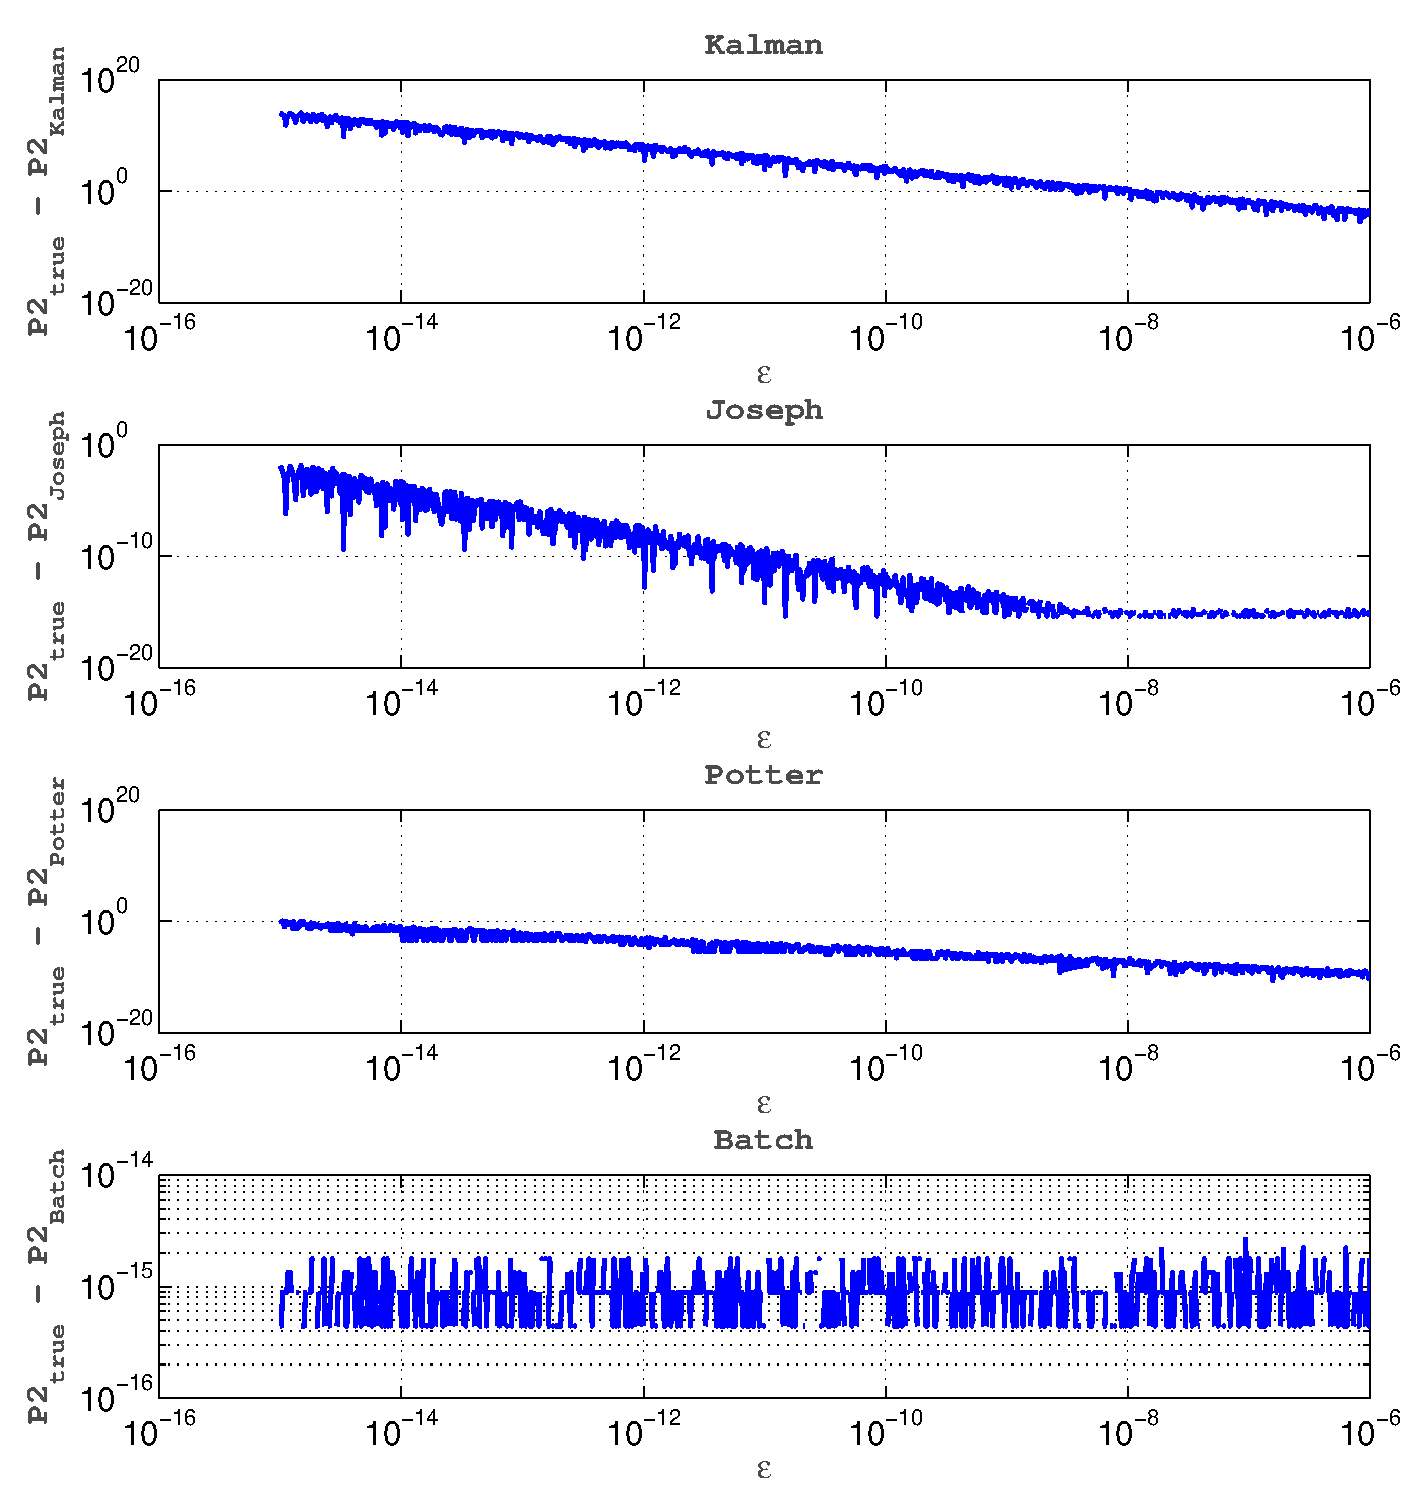
\includegraphics [width=4in]{html/HW8main_02.eps}

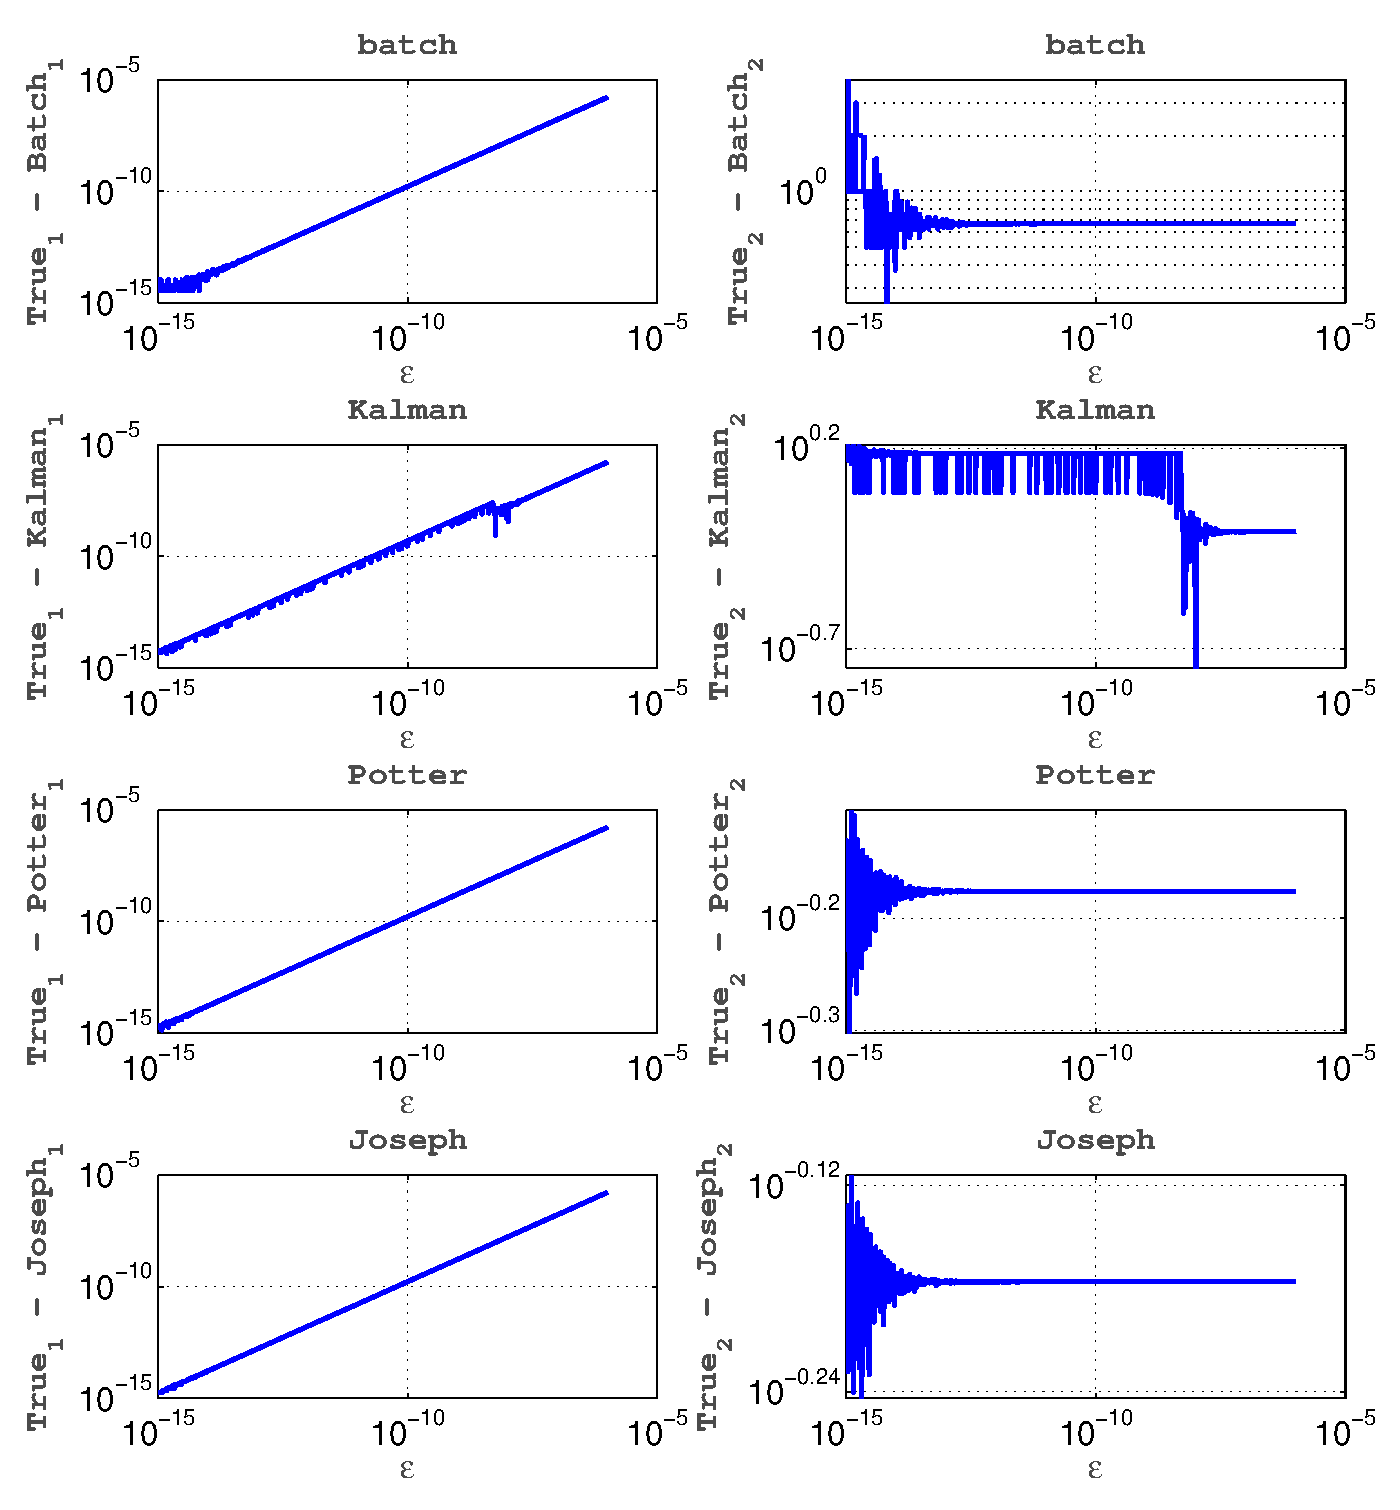
\includegraphics [width=4in]{html/HW8main_03.eps}

\vspace{3in}


\begin{lstlisting}

    

function [P2_True,P2_Kalman,P2_Joseph,P2_Potter,P2_Batch]=FindP2(e,tr)
% Compute P2 (or the trace therof) for various different algorithms. 

% Input is error value, and 'tr', indicator to return the trace of each 
%       calculation


if exist('tr','var')
    tr=1;
else 
    tr = 0;
end
    
% Return the trace!
% eq 4.7.20
% z1 = |1 3||x1| + |v1|
% z2 = |1 1||x2| + |v2|

% Looks like    y=Hx+e
P1bar   = (1/e^2)*eye(2,2);
H1      = [1 e];
H2      = [1 1];
R       = 1;
%------------------------------------------------------------
%% a - True Solution from 4.7.24

B   = 1 - 2*e + 2*e^2*(2+e^2);
P2_True  = 1/B*[ 1+2*e^2     -(1+e); ...
                  -(1+e)       2+e^2 ];
if tr              
    P2_True     = trace(P2_True);
end
%------------------------------------------------------------

%% b - P2 Using Conventional Kalman Filter
K1 = P1bar*H1'*inv(H1*P1bar*H1' + R);
P1 = (eye(2) - K1*H1)*P1bar;

% Now again for P2
K2          = P1*H2'*inv(H2*P1*H2' + R);
P2_Kalman   = (eye(2) - K2*H2)*P1;

% P2_Kalman =  1/(1-2*e)*[   -1  1; ...
%                          1   -1];
if tr
    P2_Kalman    = trace(P2_Kalman);
end
% matlabFunction(P2_Kalman,'file','P2_Kalman.m');   

%------------------------------------------------------------

%% c - P2 Using Joseph Formulation
% Branching off of the Kalman
K1          = P1bar*H1'*inv(H1*P1bar*H1' + R);
P1          = (eye(2) - K1*H1)*P1bar*(eye(2)-K1*H1)' + K1*R*K1';
K2          = P1*H2'*inv(H2*P1*H2' + R);

P2_Joseph   = (eye(2) - K2*H2)*P1*(eye(2)-K2*H2)' + K2*R*K2';
if tr
    P2_Joseph     = trace(P2_Joseph);         
end

%------------------------------------------------------------

%% d - P2 Using Plotter Algorithm (5.7.17) 

W1bar   = (chol(P1bar))';

Ftilde  = W1bar'*H1';
alpha   = inv(Ftilde'*Ftilde + R);
gamma   = 1./(1 + sqrt(R*alpha));
K       = alpha*W1bar*Ftilde;
% xhat    = xbar + K*([v1;v2]);
W1      = W1bar - gamma*K*Ftilde';
P1      = W1*W1';

% Now for obs 2
W2bar   = chol(P1)';
Ftilde  = W2bar'*H2';
alpha   = inv(Ftilde'*Ftilde + R);
gamma   = 1./(1 + sqrt(R*alpha));
K       = alpha*W2bar*Ftilde;
% xhat    = xbar + K*([v1;v2]);
W2      = W2bar - gamma*K*Ftilde';

P2_Potter = W2*W2';
if tr
    P2_Potter     = trace(P2_Potter);
end

%------------------------------------------------------------

%% e - P2 Using Batch
H       = [1 e;1 1];        %H       = [1 e; 1 1];   
R       = eye(2,2);            %   eye(2,2);      % E(ee')
P2bar   = (1/e)^2*eye(2,2);
Delta   = P2bar\eye(2,2);
Delta   = Delta + transpose(H)*inv(R)*H;

P2_Batch= Delta\eye(2,2);
if tr
    P2_Batch= trace(P2_Batch);
end
 \end{lstlisting}





\vspace{3in}

\begin{lstlisting}
function [X_batch,X_Kalman,X_Joseph,X_Potter,X_True] = FindStateP4(e)
% Return state calculations with various algorithms for homework 8,
% problem 4. 


%% b - Estimate State
Xbar    = [4 2]';
X       = [3 1]'; % True state. Use as observations  
X_True  = X';

%------------------------------------------------------
% Batch Processor
% Xhat    = (H'*inv(R)*H + inv(P1))\(H'*inv(R)*
H       = [1 2*e;1 3*e];
R       = eye(2,2);
P0bar   = (1/e^2)*eye(2,2);
Y       = H*X;
X_batch = inv(H'*inv(R)*H + inv(P0bar))*(H'*inv(R)*Y + inv(P0bar)*Xbar);
X_batch = X_batch';


%------------------------------------------------------
% Kalman Filter - Think of the two observations as occuring at different
% times. With the first becoming a-priori for the next one
H1          = H(1,:);
H2          = H(2,:);
R1          = 1; R2 = R1;
P1bar       = P0bar; 

K1          = P1bar*H1'*inv(H1*P1bar*H1' + R1);
P1_1        = (eye(2) - K1*H1)*P1bar;
X1_Kalman   = Xbar + K1*(Y(1) - H1*Xbar);

% Now again for number 2. The X1_Kalman state is now the a-priori for the
% new state
K2          = P1_1*H2'*inv(H2*P1_1*H2' + R2);
P2_Kalman   = (eye(2) - K2*H2)*P1_1;
X2_Kalman   = X1_Kalman + K2*(Y(2) - H2*X1_Kalman);

X_Kalman    = X2_Kalman';


%------------------------------------------------------
% Joseph Formulation
K1          = P1bar*H1'*inv(H1*P1bar*H1' + R1);
P1          = (eye(2) - K1*H1)*P1bar*(eye(2)-K1*H1)' + K1*R1*K1';
X1_Joseph   = Xbar + K1*(Y(1) - H1*Xbar);

P2bar       = P1;
K2          = P1*H2'*inv(H2*P1*H2' + R2);
P2          = (eye(2) - K2*H2)*P2bar*(eye(2)-K2*H2)' + K2*R2*K2';
X2_Joseph   = X1_Joseph + K2*(Y(2) - H2*X1_Joseph);

X_Joseph    = X2_Joseph';


%------------------------------------------------------
% Potter Algorithm
W1bar       = (chol(P0bar))';

Ftilde      = W1bar'*H1';
alpha       = inv(Ftilde'*Ftilde + R1);
gamma       = 1./(1 + sqrt(R1*alpha));
K1          = alpha*W1bar*Ftilde;
% xhat    = xbar + K*([v1;v2]);
W1          = W1bar - gamma*K1*Ftilde';
P1          = W1*W1';
X1_Potter   = Xbar + K1*(Y(1) - H1*Xbar);

% Now for obs 2
W2bar       = chol(P1)';
Ftilde      = W2bar'*H2';
alpha       = inv(Ftilde'*Ftilde + R2);
gamma       = 1./(1 + sqrt(R2*alpha));
K2          = alpha*W2bar*Ftilde;
% xhat    = xbar + K*([v1;v2]);
W2          = W2bar - gamma*K2*Ftilde';
P2_Potter   = W2*W2';
X2_Potter   = X1_Potter + K2*(Y(2) - H2*X1_Potter);


X_Potter    = X2_Potter';




\end{lstlisting}











\end{document}